% Chapter 1

\chapter{Introducción General} % Main chapter title

\label{Chapter1} % For referencing the chapter elsewhere, use \ref{Chapter1} 
\label{IntroGeneral}
En este capítulo se presenta una breve introdución a la plataforma CIAABOT, y se
explica la necesidad que dio origen a desarrollar este proyecto. También se detallan
los motivos que llevaron a realizarlo, cuáles son los objetivos y el alcance.

%----------------------------------------------------------------------------------------

% Define some commands to keep the formatting separated from the content 
\newcommand{\keyword}[1]{\textbf{#1}}
\newcommand{\tabhead}[1]{\textbf{#1}}
\newcommand{\code}[1]{\texttt{#1}}
\newcommand{\file}[1]{\texttt{\bfseries#1}}
\newcommand{\option}[1]{\texttt{\itshape#1}}
\newcommand{\grados}{$^{\circ}$}

%----------------------------------------------------------------------------------------

%\section{Introducción}

%----------------------------------------------------------------------------------------
\section{Introducción}
\label{Introducción}
En el presente trabajo se describe la implementación de un \emph{debugger} interactivo
para CIAABOT IDE (IDE son las siglas en inglés de entorno de desarrollo integrado). CIAABOT es una plataforma de software y hardware abierto que forma parte del proyecto CIAA (Computadora Industrial Abierta Argentina) \citep{CIAA}. 


La implementacion de este trabajo tiene la misión de contribuir a la formación
académica de los alumnos, así como también brindar un aporte al proyecto CIAA, mediante el agregado de capacidad de depuración a los programas desarrollados con CIAABOT IDE.

En la sección \ref{CIAABOT} se introduce el proyecto CIAABOT y las partes que lo componen; también se listan los pasos que son parte del flujo de trabajo en el IDE.
En la sección \ref{Debug y Debugger} se exponen los conceptos involucrados en el contexto del desarrollo del presente proyecto, y en la sección \ref{Motivación} se introducen los motivos que llevaron a realizarse. Por último, en la sección \ref{Objetivos y alcance} se presentan los objetivos propuestos y el alcance.


\subsection{CIAABOT}
\label{CIAABOT}

CIAABOT es una plataforma de robótica educativa. Tiene como propósito principal introducir
de forma sencilla la programación de robots.

Las partes componentes que lo integran son:

\begin{itemize}
	\item CIAABOT IDE: es un entorno de programación en lenguaje CIAABOT (basado en  Blockly \citep{blockly}), que es un lenguaje gráfico donde un programa se crea encastrando bloques. Permite crear el programa, compilarlo y descargarlo a las plataformas de hardware.
	\item CIAABOTS: son las plataformas de hardware que se programan desde CIAABOT IDE. 
	\item Firmware: el programa creado en CIAABOT IDE genera internamente código C que se combina con el firmare pre-existente del proyecto CIAA y se compila para su posterior descarga a la plataforma.
\end{itemize}

Se observa en la figura \ref{fig:editor} el área en dónde se desarrolla el flujo de trabajo, las cuales son:

\begin{enumerate}
	\item Armar un programa: encastrando bloques predifinidos por
	la plataforma.	
	\item Visualizar el código generado en C: actualizado en tiempo real cuando se
	manipulan los bloques.
	\item Compilar: a partir del código sintácticamente correcto se traduce al código
	para usar en la placa.
	\item Descargar: instalar el código generado en la plataforma de hardware.
	\item Usar la placa con el programa: comenzar a realizar los ensayos sobre la placa.
\end{enumerate}

\begin{figure}[h]
	\centering
	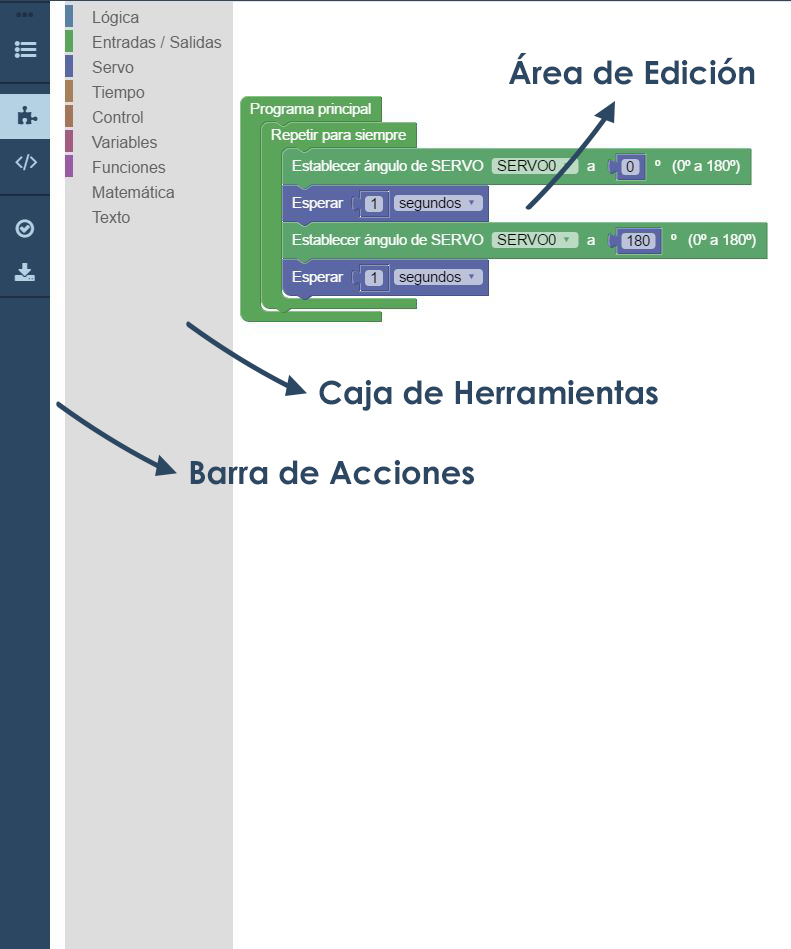
\includegraphics[scale=.50]{./Figures/editor.PNG}
	\caption{Área de flujo de trabajo de CIAABOT-IDE.}
	\label{fig:editor}
\end{figure}

\subsection{\emph{Debug} y \emph{Debugger}}
\label{Debug y Debugger}

El depurador es un programa que ejecuta ciertas rutinas de código de otros programas (programa objetivo), con el fin de encontrar y eliminar errores. Esta técnica permite al código ser examinado y obtener información sobre el estado en el que se está ejecutando.

Mediante el proceso de depuración de programas, se puede identificar y corregir errores propios de programación, corriendo un programa paso a paso, parandolo o pausandolo, de esta manera se realiza el seguimiento de
valores de las variables, dando en consecuencia la posibilidad al programador
de corregir errores y pulir el funcionamiento de su programa.

Como el software en general y los sistemas electrónicos se vuelven generalmente
más complejos, se da importancia al desarrollo de técnicas y herramientas de depuración,
precisamente por las ventajas que tiene, como son el detectar anomalías
en cada paso, corregir y mejorar las funcionalidades. 

%----------------------------------------------------------------------------------------

\section{Motivación}
\label{Motivación}

La plataforma CIAABOT no posee la capacidad de \emph{debuggear} un programa.
Para realizar los ensayos se tiene que compilar el programa, descargalo y luego manualmente probar la lógica en la placa usando, como por ejemplo, los leds, botones, mensajes por UART, etc.

Se plantea el desarrollo de un \emph{debugger} interactivo para CIAABOT debido a la
importancia de realizar pruebas de un programa en tiempo real y de esta manera verificar la lógica del programa.

El desarrollo del \emph{debugger} interactivo para CIAABOT seguirá los lineamientos
de diseño de CIAABOT implementando el desarrollo con una visión de
fácil utilización, simple e intuitivo, teniendo en cuenta quienes serán los usuarios
finales.

Se aprovechará con el desarrollo de esta implementación poder aplicar todos los
conocimientos aprendidos durante la carrera de especialización de sistemas embebidos.


%----------------------------------------------------------------------------------------

\section{Objetivos y alcance}
\label{Objetivos y alcance}

El objetivo de este proyecto es brindarle al usuario una herramienta útil para la
corrección e identificación de los errores de programación cuando está usando
la plataforma CIAABOT. Para lograrlo se pretende desarrollar un \emph{debugger} para
CIAABOT que cumpla con las siguientes características: 

\begin{itemize}
	\item Ejecutar un programa bloque por bloque.
	\item Detener la ejecución temporalmente en un bloque encastrable concreto.
	\item Visualizar el contenido de las variables en un determinado momento de la
	ejecución.
	\item Entorno gráfico amigable.
	\item Importar el programa de bloques creado en el IDE de desarrollo de CIAABOT.	
\end{itemize}

De esta manera el aprendizaje del usuario programador primerizo será más enriquesedor,
identificando y subsanando los errores de ejecución.

%----------------------------------------------------------------------------------------






